\documentclass[11pt]{article}

\usepackage[margin=1in]{geometry}
\usepackage{amsmath, amssymb, amsthm, mathtools, bm}
\usepackage{graphicx, float, subcaption}
\usepackage{booktabs}
\usepackage{enumitem}
\usepackage{multicol}
\usepackage[hidelinks]{hyperref}

\graphicspath{{../output/}}

\newcommand{\E}{\mathbb{E}}
\newcommand{\R}{\mathbb{R}}
\DeclareMathOperator{\diag}{diag}

\title{ECON 880: Problem Set 1 (Lentz)\\[2pt] \large Rust (1987), Zurcher's bus engine replacement}
\author{Arthur Maur\'icio Rodrigues}
\date{\today}

\begin{document}
\maketitle

%==============================================================================
\section*{Question 1}
%==============================================================================

The log-likelihood is additively separable in $(\mu,\sigma)$ (present in $O$) and $h$ (present in $R$). First-order conditions for $O$ yield:

\paragraph{Odometer process.}
\begin{align*}
  \frac{\partial O}{\partial \mu} &= \sum_{i,s} \frac{\ln\Delta x_{is} - \mu}{\sigma^2} = 0
    &&\Longrightarrow\quad \hat\mu = \frac{1}{M}\sum_{i,s}\ln\Delta x_{is},\\
  \frac{\partial O}{\partial \sigma} &= \sum_{i,s}\left[\frac{(\ln\Delta x_{is} - \mu)^2}{\sigma^3} - \frac{1}{\sigma}\right] = 0
    &&\Longrightarrow\quad \hat\sigma^2 = \frac{1}{M}\sum_{i,s}\left(\ln\Delta x_{is} - \hat\mu\right)^2.
\end{align*}


Let $K_n = \sum_{i,s}\chi_{isn}$ be the bus-months that start in bin $n$, and let $D_n = \sum_{i,s}\chi_{isn}\,d_{i,s+1}$ the replacements among them.
\[
  R(Y\mid\bm h) = \sum_{n=1}^{N}\Big[D_n\ln h_n + (K_n - D_n)\ln(1-h_n)\Big],
\]

\[
  \frac{D_n}{h_n} - \frac{K_n - D_n}{1-h_n} = 0
  \quad\Longrightarrow\quad
  \hat h_n = \frac{D_n}{K_n}.
\]

\paragraph{Estimates.}
\begin{align*}
  \hat\mu &= 8.0158 \quad (e^{\hat\mu} \approx 3{,}030 \text{ miles in a median month}), &
  \hat\sigma &= 0.6321,\\
  O(Y\mid\hat\theta) &= -71{,}961.20, &
  R(Y\mid\hat\theta) &= -284.44,\\
  \mathcal{L}(Y\mid\hat\theta) &= -72{,}245.63. &&
\end{align*}

\begin{figure}[H]
  \centering
  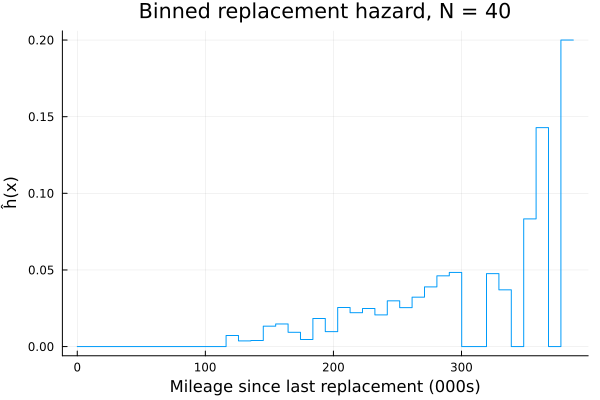
\includegraphics[width=0.75\textwidth]{hazard_binned.png}
  \caption{Binned replacement hazard, $N = 40$.}
  \label{fig:binned}
\end{figure}

\begin{figure}[H]
  \centering
  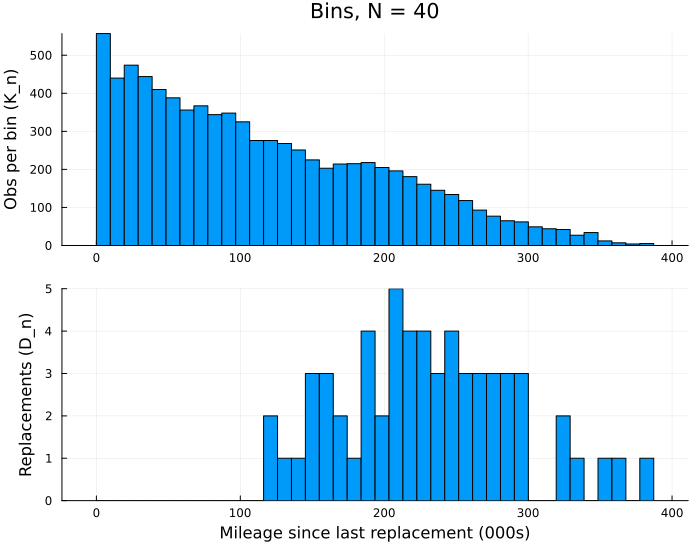
\includegraphics[width=0.75\textwidth]{bins.png}
  \caption{Bus-months ($K_n$, top) and replacements ($D_n$, bottom) by mileage bin.}
  \label{fig:bins}
\end{figure}

\begin{table}[H]
  \centering
  \small
  \caption{Binned hazard estimates. Mileage in thousands.}
  \label{tab:bins}
  \begin{minipage}[t]{0.48\textwidth}
    \centering
    \begin{tabular}{rrrrrr}
      \toprule
      $n$ & $\bar x_{n-1}$ & $\bar x_n$ & $K_n$ & $D_n$ & $\hat h_n$ \\
      \midrule
      1 & 0.0 & 9.7 & 557 & 0 & 0.0000 \\
      2 & 9.7 & 19.4 & 440 & 0 & 0.0000 \\
      3 & 19.4 & 29.0 & 474 & 0 & 0.0000 \\
      4 & 29.0 & 38.7 & 444 & 0 & 0.0000 \\
      5 & 38.7 & 48.4 & 410 & 0 & 0.0000 \\
      6 & 48.4 & 58.1 & 388 & 0 & 0.0000 \\
      7 & 58.1 & 67.8 & 356 & 0 & 0.0000 \\
      8 & 67.8 & 77.5 & 367 & 0 & 0.0000 \\
      9 & 77.5 & 87.1 & 344 & 0 & 0.0000 \\
      10 & 87.1 & 96.8 & 348 & 0 & 0.0000 \\
      11 & 96.8 & 106.5 & 325 & 0 & 0.0000 \\
      12 & 106.5 & 116.2 & 276 & 0 & 0.0000 \\
      13 & 116.2 & 125.9 & 276 & 2 & 0.0072 \\
      14 & 125.9 & 135.5 & 268 & 1 & 0.0037 \\
      15 & 135.5 & 145.2 & 251 & 1 & 0.0040 \\
      16 & 145.2 & 154.9 & 225 & 3 & 0.0133 \\
      17 & 154.9 & 164.6 & 203 & 3 & 0.0148 \\
      18 & 164.6 & 174.3 & 214 & 2 & 0.0093 \\
      19 & 174.3 & 184.0 & 215 & 1 & 0.0047 \\
      20 & 184.0 & 193.6 & 218 & 4 & 0.0183 \\
      \bottomrule
    \end{tabular}
  \end{minipage}\hfill
  \begin{minipage}[t]{0.48\textwidth}
    \centering
    \begin{tabular}{rrrrrr}
      \toprule
      $n$ & $\bar x_{n-1}$ & $\bar x_n$ & $K_n$ & $D_n$ & $\hat h_n$ \\
      \midrule
      21 & 193.6 & 203.3 & 205 & 2 & 0.0098 \\
      22 & 203.3 & 213.0 & 196 & 5 & 0.0255 \\
      23 & 213.0 & 222.7 & 181 & 4 & 0.0221 \\
      24 & 222.7 & 232.4 & 161 & 4 & 0.0248 \\
      25 & 232.4 & 242.1 & 145 & 3 & 0.0207 \\
      26 & 242.1 & 251.7 & 134 & 4 & 0.0299 \\
      27 & 251.7 & 261.4 & 118 & 3 & 0.0254 \\
      28 & 261.4 & 271.1 & 93 & 3 & 0.0323 \\
      29 & 271.1 & 280.8 & 77 & 3 & 0.0390 \\
      30 & 280.8 & 290.5 & 65 & 3 & 0.0462 \\
      31 & 290.5 & 300.1 & 62 & 3 & 0.0484 \\
      32 & 300.1 & 309.8 & 49 & 0 & 0.0000 \\
      33 & 309.8 & 319.5 & 44 & 0 & 0.0000 \\
      34 & 319.5 & 329.2 & 42 & 2 & 0.0476 \\
      35 & 329.2 & 338.9 & 27 & 1 & 0.0370 \\
      36 & 338.9 & 348.6 & 34 & 0 & 0.0000 \\
      37 & 348.6 & 358.2 & 12 & 1 & 0.0833 \\
      38 & 358.2 & 367.9 & 7 & 1 & 0.1429 \\
      39 & 367.9 & 377.6 & 4 & 0 & 0.0000 \\
      40 & 377.6 & 387.3 & 5 & 1 & 0.2000 \\
      \bottomrule
    \end{tabular}
  \end{minipage}
\end{table}

%==============================================================================
\section*{Question 2: Bernstein hazard}
%==============================================================================

\[
  h(x\mid \bm f) = \sum_{k=1}^{n} f_k\, b_{k,n}(u), \qquad b_{k,n}(u) = \binom{n}{k} u^k (1-u)^{n-k},
\]

\begin{align*}
  R(\bm f) &= \sum_i \Big[d_i \ln h_i + (1-d_i)\ln(1-h_i)\Big],\\
  \nabla R(\bm f) &= B^\top \bm w, & w_i &= \frac{d_i}{h_i} - \frac{1-d_i}{1-h_i},\\
  \nabla^2 R(\bm f) &= -B^\top \diag(\bm v)\, B, & v_i &= \frac{d_i}{h_i^2} + \frac{1-d_i}{(1-h_i)^2}.
\end{align*}

\[
  \hat{\bm f} = (0,\ 0,\ 0.00465,\ 0.0710,\ 0.0379), \qquad R(\hat{\bm f}) = -298.2855, \qquad \mathcal{L}(Y\mid\hat\theta) = -72{,}259.48.
\]

\begin{figure}[H]
  \centering
  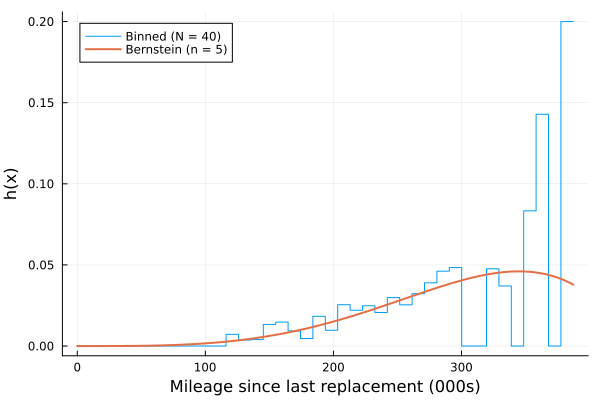
\includegraphics[width=0.75\textwidth]{hazard_bern.png}
  \caption{Bernstein hazard ($n=5$) over the binned estimate.}
  \label{fig:bern}
\end{figure}

\subsection*{(a) Newton--Raphson}

\subsection*{(b) Nelder--Mead}

\subsection*{(c) Nelder--Mead, then Newton--Raphson}

\subsection*{(d) Summary}

\begin{table}[H]
  \centering
  \caption{Performance across 24 starting values.}
  \label{tab:methods}
  \small
  \begin{tabular}{lcccc}
    \toprule
    Method & At optimum & Reports converged & Worst gap in $R$ & Median iter. \\
    \midrule
    Newton--Raphson                    & 0/24  & 0/24  & 15{,}792 & 26 \\
    Projected Newton--Raphson          & 24/24 & 24/24 & $<10^{-10}$ & 12.5 \\
    Nelder--Mead                       & 0/24  & 24/24 & 2{,}511  & 833 \\
    Nelder--Mead with restarts         & 10/24 & 24/24 & 15.8     & 1{,}671 \\
    NM (50 iter.) $\to$ NR             & 0/24  & 0/24  & 8{,}498  & 74 \\
    NM (50 iter.) $\to$ projected NR   & 24/24 & 24/24 & $<10^{-10}$ & 61 \\
    \bottomrule
  \end{tabular}
\end{table}

\end{document}
